\chapter{Analyse vorhandener Daten}
\label{chap:kapitel4}

Ein Modell, welches beim Data Mining genutzt werden kann, ist das \ac*{CRISP-DM}. Diese Modell definiert das Data Mining als Prozess mit sechs verschiedenen Phasen und kann der 
Abbildung \ref*{fig:CRISP-DM} entnommen werden. Dabei dürfen diese Phasen nicht als starr aufeinander folgend betrachtet werden. Denn auch Erkenntnisse aus nachfolgende Phasen können vorherige Phasen
beeinflussen, was deutlich wird, durch die Pfeile zwischen den Phasen in der Abbildung \ref*{fig:CRISP-DM}. In der ersten Phase, dem Business Understanding, liegt der Schwerpunkt auf dem Verständnis 
der Projektziele aus der Geschäftsperspektive. Mit dem erlangten Wissen daraus, kann eine Data-Mining Problemstellung definiert werden, wie dies in Kapitel \ref*{chap:Zielsetzung} erfolgt ist. 
Die nächste Phase ist das Data Understanding. Diese Phase beschäftigt sich mit der ersten Datenerhebung und dem Aufbau eines Datenverständnisses. Zudem wird in dieser Phase versucht mögliche Probleme 
bei der Qualität der Daten zu identifizieren. Nach der Phase des Data Understandings folgt die Phase der Data Preparation. Während dieser Phase ist das Ziel die Rohdaten so aufzubereiten, dass ein 
Datensatz dabei erstellt wird, der für eine Modellierung geeignet ist \cite[S.5-7]{q8}. Die nächsten drei Phasen beschäftigen sich mit der Modellierung, der Evaluierung von Modellen und dem Einsatz 
eines Modells und gehen somit über die Aufgabenstellung des Praxisprojekt hinaus und werden deshalb im Folgenden nicht berücksichtigt.

\begin{figure}[H]
    \centering
    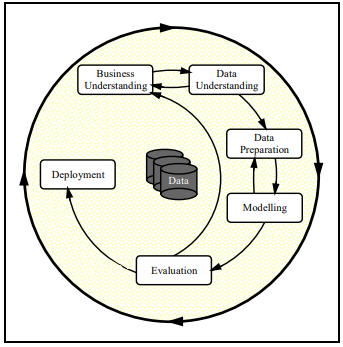
\includegraphics[]{abbildungen/CrispDM.PNG}
    \caption{\ac*{CRISP-DM} Phasen \cite[S.5]{q8}}
    \label{fig:CRISP-DM}
\end{figure}

